\chapter{ESTUDO DE CASO}
Este capítulo apresenta um estudo de caso da implementação de uma ferramenta de documentação executável no projeto da Biblioteca Digital.

O estudo de caso foi idealizado visando comprovar as vantagens obtidas na produção e uso de documentação executável. Espera-se que o uso deste recurso no presente trabalho, traga como valores o apoio a validação de requisitos e maiores facilidades para treinamento de usuários no emprego do sistema.

\section{Projeto da Biblioteca Digital}

A Biblioteca Digital (BD) é um projeto de pesquisa e desenvolvimento que inciou-se em março de 2007, através de uma solicitação da SETEC/MEC ao Núcleo de Pesquisa de Sistemas de Informação (NSI) do Instituto Federal Fluminense. O NSI foi criado em abril de 2002 e desde essa época vem estimulando o uso tecnologias livres para pesquisa e desenvolvimento de software.

O projeto da BD visa disponibilizar um acervo de documentos produzidos pela rede de Instituições de Educação Profissional Científica e Tecnológica (EPCT) – como artigos, monografias, dissertações, teses e periódicos – promovendo a disseminação de conhecimento através destes conteúdos.

Como em todo projeto de desenvolvimento de software, a documentação do sistema é um problema constante. Sincronizar documentos escritos em papel com o código do sistema, é uma tarefa difícil e sujeita a falhas.

\section{Proposta da ferramenta}

Devido a este problema, foi levantada a necessidade de desenvolver uma ferramenta de documentação executável, denominada NSI-BD-Tour, que permita ao usuário validar requisitos do sistema e guiá-lo na utilização do mesmo. Portanto esta ferramenta tem como objetivos suportar sua documentação e treinar o usuário no emprego do sistema.

O NSI-BD-Tour deve suportar o cadastro de cenários, em um formato pré-estabelecido, com a descrição passo a passo de uma funcionalidade específica do sistema. A ferramenta então, deve ser capaz de executar esse cenário, guiando o usuário até a conclusão do mesmo. Isto é, indicar ao usuário, quais ações ele deve fazer, como clicar em um determinado botão ou preencher um campo de texto, a fim de atingir o objetivo final.

Assim, pode-se destacar como vantagens da implantação a otimização do uso do sistema, pois através dos passos estabelecidos o usuário poderá avaliar a simplicidade da execução das ações ou estabelecer outros comportamentos melhorados.

Outra vantagem esperada é a validação dos cenários, onde todos os passos executados foram pré-definidos pela especificação do cliente. Desta maneira pode-se validar interativamente todos os cenários descritos.

A partir da utilização da documentação interativa, os usuários poderão ser facilmente treinados nas funcionalidades da Biblioteca Digital, sem a necessidade de uma tutoria dedicada.

\section{Desenvolvimento}

Neste tópico serão demonstrados os passos executados para realização deste trabalho, possibilitando ao leitor avaliar ou reproduzir os efeitos aqui descritos.

\subsection{Ambiente de desenvolvimento}

O projeto da BD é desenvolvido na linguagem \textit{Ruby} utilizando o \textit{framework} \textit{web Ruby on Rails} \cite{RAILS}. Uma das vantagens de utilizar este \textit{framework} é a existência de um conjunto de bibliotecas que facilitam o desenvolvimento guiado a testes \cite{BECK}.

Durante o processo de desenvolvimento da ferramenta foi utilizada a biblioteca de testes automatizados RSpec \cite{CHELIMSKY}, a qual fornece ao desenvolvedor uma \textit{domain specific language} (DSL), que facilita especificação dos comportamentos esperados do objeto (Código \ref{lst:codigo31}).

{\singlespace
\begin{lstlisting}[caption=Exemplo da DSL do Rspec,label={lst:codigo31}]
describe Person do
  subject {
    Person.new(:name => "John Doe", :role => "moderator")
    }

  its(:name) { should == "John Doe" }

  it "is a admin" do
    subject.role = "admin"
    subject.should be_admin
  end

  it "is not a admin" do
    subject.role = nil
    subject.should_not be_admin
  end

  it "instantiates without hash" do
    expect { Person.new }.to_not raise_error(ArgumentError)
  end
end
\end{lstlisting}
}

O resultado de execução do código acima pode ser visto na Figura \ref{figura_31}, a qual descreve os testes que passaram.

\begin{figure}[ht]
    \centering
    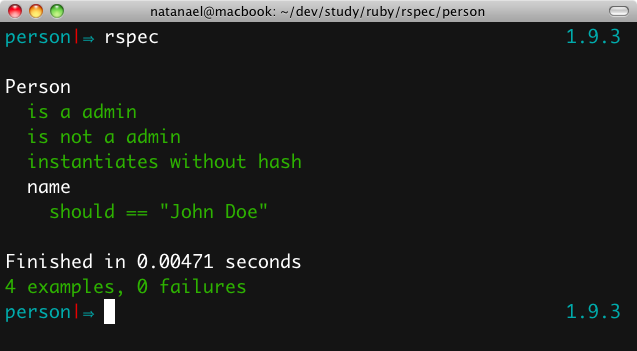
\includegraphics[width=0.9 \textwidth]{figuras/figura_31}
    \caption{Saída após rodar os testes com RSpec}
    \label{figura_31}
\end{figure}

Além da utilização desta biblioteca de testes, foi utilizado o conceito de "passos de bebê", ou seja, pequenas partes são desenvolvidas a cada momento, seja levantamento de requisitos, implementação de funcionalidade, refatoração ou até especificações. Um exemplo disto é focar no desenvolvimento de uma pequena parte de uma funcionalidade, diminuindo o risco do desenvolvimento e asegurando o atingimento de objetivos alcançaveis \cite{RODRIGO}.















\section{Arquitetura da ferramenta}

A proposta inicial para ferramenta NSI-BD-Tour foi a construção de uma arquitetura onde os elementos constituintes eram o cenário (funcionalidade), passos (etapas) e ações (executas em cada passo), os quais se relacionavam conforme o modelo apresentado na Figura \ref{figura_32}.

\begin{figure}[ht]
    \centering
    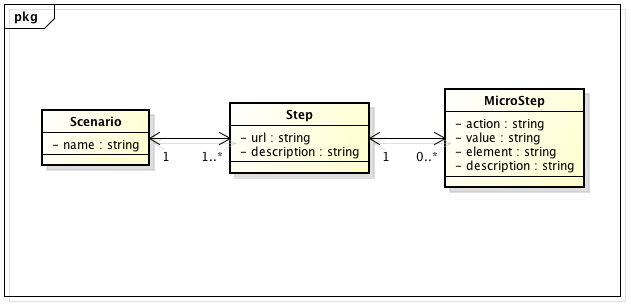
\includegraphics[width=0.5 \textwidth]{figuras/figura_32}
    \caption{Diagrama de classes da arquitetura inicial}
    \label{figura_32}
\end{figure}

Entretanto, após implementada esta arquitetura pode-se verificar a dificuldade na utilização da ferramenta. Implementada desta maneira, o NSI-BD-Tour iria gerar um grande trabalho no processo de cadastro de \textit{Steps} e \textit{MicroSteps}, as quais são muito utilizadas devido a existência de vários passos e ações a serem executadas em um único cenário.

Com este problema, foi realizado um refatoramento que levou a descoberta de uma biblioteca da linguagem \textit{Ruby} (\textit{Hashr}) que facilitou uma nova arquitetura. A biblioteca \textit{Hashr} cria uma nova classe derivada da classe \textit{Hash} (estrutura de dicionário), que simplifica o acesso aos valores de dicionários aninhados \cite{HASHR}. O Código \ref{lst:codigo36} exemplifica o uso desta estrutura.

{\singlespace
\begin{lstlisting}[caption=Exemplo de uso da estrutura \textit{Hashr},label={lst:codigo36}]
monografia = Hashr.new titulo: 'Documentacao Executavel',
                       autores: {autor_1: 'Tiago', autor_2: 'Natanael'}

monografia.titulo  # => 'Documentacao Executavel'
monografia.autor_1 # => 'Tiago'
monografia.autor_2 # => 'Natanael'

\end{lstlisting}
}

A linha 1 do código acima, cria uma instância da classe \textit{Hashr}. Pode-se verificar que o parâmetro recebido é um dicionário nativo (\textit{Hash}). Após criado o objeto, é possivel visualizar nas linhas 4, 5 e 6 as vantagens da utilização desta biblioteca. Os valores podem ser acessados diretamente pelo valor da chave, como atributos.

Através das vantagens descobertas, foi possível fazer a simplificação da entrada de dados para o cadastro e gerenciamento dos cenários, utilizando o formato de serialização de dados YAML, o qual permite descrever em forma textual todos os dados necessários para ferramenta funcionar, eliminando a necessidade de preencher vários formulários.

Por fim, após toda a estrutura de dados criada, será necessário criar a interface de interação com usuário, utilizando a biblioteca \textit{Amberjack2} e jQuery. Desta maneira, o cenário poderá ser executado, realizando na validação e treinamento do usuário.

\section{Funcionalidades desenvolvidas}

Nesta seção serão descritas as funcionalidades especificadas para o desenvolvimento da ferramenta NSI-BD-Tour.

\textbf{F01.} Cadastro e gerenciamento de cenários

O objetivo desta funcionalidade é permitir o usuário descrever os cenários em uma linguagem simples - formato YAML. O cenário descrito será utilizado para validar e guiar o usuário no emprego do sistema. Na implementação dessa funcionalidade, foi criado um cadastro de cenários, onde há um campo de texto em que o usuário pode descrever o cenário.

Para implementar esta funcionalidade, utilizou-se de um recurso disponibilizado pelo \textit{framework} (\textit{Rails}) no qual a Biblioteca Digital é desenvolvida. O Código \ref{lst:codigo42} representa o comando utilizado para criar o modelo definido.

{\singlespace
\begin{lstlisting}[caption=Comando para gerar um modelo,label={lst:codigo42}]
$ rails generate scaffold Scenario yaml:text
\end{lstlisting}
}

Após executar o comando, é criada uma classe \textit{Scenario} com o atributo yaml, a qual será responsável pela manipulação dos cenários do sistema. Além disso, este comando também gera toda interface de gerenciamento para o usuário.

Uma limitação desta funcionalidade ainda não abordada é a validação do formato do texto inserido pelo usuário. Caso o cenário inserido não atenda ao padrão, poderá comprometer o funcionamento da ferramenta.

\textbf{F02.} Análise e extração de dados

Através do cadastro de cenários (funcionalidade F01) o usuário poderá cadastrá-los, utilizando o formato YAML. Porém o cenário está descrito em forma textual, e precisa ser processado para a extração das informações necessárias para o funcionamento da ferramenta. O objetivo da análise e extração de dados do YAML é obter os atributos necessários para renderização no navegador.

Para converter o YAML em uma estrutura manipulável, foi utilizada a biblioteca \textit{Psych} \cite{PSYCH}. Esta biblioteca fornece uma maneira simples de se transformar um texto em formato YAML para uma estrutura nativa do \textit{Ruby}, composta por dicionários, listas e valores simples (Código \ref{lst:codigo38}).

{\singlespace
\begin{lstlisting}[caption=Exemplo de cenário escrito em \textit{YAML},label={lst:codigo38}]
require "psych"

yaml = <<-YAML
scenario: Login de Usuario

contexts:
  - url: /
    steps:
      - description:
          Os links referentes ao acesso do usuario
          ficam no menu do canto superior direito
        element: actions
        padding: 3
        position: rmb

      - description: Clique na opcao 'Acesso'
        element: sign_in
        padding: 3
        position: rmb
        action: click
YAML

cenario = Psych.load(yaml)
\end{lstlisting}
}

Nas linhas 3-21 foi definido um texto em formato YAML, o qual será convertido para uma estrutura manipulável e nativa da linguagem \textit{Ruby} utilizando a biblioteca \textit{Psych} (linha 23).

Por fim, para implementar esta funcionalidade, foi desenvolvido um método responsável pela conversão dos dados obtidos do cenário textual, para estrutura \textit{Hashr}. A classe \textit{Scenario}, criada na funcionalidade F01, receberá o método (Código \ref{lst:codigo37}) que possibilitará o NSI-BD-Tour converter todos os cenários uma estrutura que facilita o acesso aos valores dos atributos.

{\singlespace
\begin{lstlisting}[caption=Método de conversão para \textit{Hashr},label={lst:codigo37}]
def convert_to_hashr(hash)
 hash = Hashr.new(hash)
 hash.values.find_all { |value| value.is_a?(Array) }.each do |value|
   value.each_index do |i|
     value[i] = convert_to_hashr(value[i]) if value[i].is_a? Hash
   end
 end
 hash
end
\end{lstlisting}
}

No código \ref{lst:codigo37}, foi criado um laço recursivo, que irá converter todos os dicionários presentes na estrutura convertida pela biblioteca \textit{Psych} (Código \ref{lst:codigo38}, linha 3). Assim, todos os valores do cenário poderão ser acessados diretamente como atributos.

\textbf{F03.} Renderização do cenário

A renderização do cenário tem como objetivo fornecer todos os dados necessários para que a biblioteca \textit{Amberjack2} possa criar e conduzir os cenários pré-cadastrados. Quando um usuário iniciar a execução de um cenário, todos os atributos devem estar na estrutura HTML interpretada pela biblioteca \textit{Amberjack2}. Assim todas páginas correspondentes a cada cenário devem conter este trecho de código descrito abaixo.

{\singlespace
\begin{lstlisting}[caption=Cenário descrito em \textit{HTML} para biblioteca \textit{Amberjack2},language=HTML,label={lst:codigo40}]
<div class="ajTourDef" id="1-tour-exemplo" style="display:none" title="/">
  <div title="http://www.exemplo.com">
    <div title="id:'elemento_id',padding:padding,trbl:'rmb'">
      Aqui vai o texto do primeiro passo
    </div>
    <div title="id:'elemento_id',padding:padding,trbl:'rmb'">
      Aqui vai o texto do segundo passo
    </div>
  </div>
</div>

\end{lstlisting}
}

O Código \ref{lst:codigo40} tem sua visualização oculta para usuário e é de uso interno da biblioteca (seção \ref{sec:amberjack}). Para ocultá-lo foi utilizada a condição da existência do parâmetro de inicialização do \textit{Amberjack2} (Código \ref{lst:codigo43}). Com isso, o trecho de código HTML estará na página quando realmente for chamado.

{\singlespace
\begin{lstlisting}[caption=Método para carregar o cenário,label={lst:codigo43}]
before_filter :load_scenario

def load_scenario
 params[:tourId] ||= cookies[:ajcookie_tourId]
 @current_scenario = Scenario.find_by_id(params[:tourId])
 cookies[:ajcookie_tourId] = @current_scenario.to_param if @current_scenario
end
\end{lstlisting}
}

O Código \ref{lst:codigo43} pertence a classe \textit{ApplicationController} (classe pai de todos os controllers do \textit{framework Rails}). A linha 1, define a obrigatoriedade de execução do método \textit{$load\_scenario$} antes de qualquer renderização. Já na linha 4, é feita verificação da existência do parâmetro. Assim, a ferramenta poderá saber qual o cenário está sendo utilizado (linha 5).

No entanto, foi detectado um problema ao passar as etapas dos cenários que sofrerem um evento do tipo redirect\footnotemark[1], por exemplo a submissão de um formulário. Neste caso, o redirect causa a perda do parâmetro na URL, deste modo a ferramenta será interrompida, devido a falta do escopo de execução.

A solução para este problema foi a utilização \textit{cookies}\footnotemark[2]. Ao iniciar o cenário, um cookie é criado para identificar qual o cenário em execução (Código \ref{lst:codigo43}, linha 6). Deste modo, o redirect não será mais um problema, e a biblioteca Amberjack2 poderá verificar a existência do \textit{cookie} e continuar executando a ferramenta.

A funcionalidade F04, descrita a seguir, irá demonstrar os passos executados para implementação do gerenciamento de \textit{cookies}.

\footnotetext[1]{Redirect é uma técnica onde é possível direcionar o acesso a outro endereço.}
\footnotetext[2]{Cookie é um grupo de dados trocados entre o navegador e o servidor. Estes dados são armazenados em um arquivo no computador do cliente.}

\textbf{F04.} Gerenciamento de cookies

O gerenciamento de cookies ficou sob a responsabilidade do \textit{Amberjack2} e do framework da Biblioteca Digital. A primeira requisição com o parâmetro na URL é responsável por iniciar a execução de um cenário e criar um cookie com os dados necessários para o \textit{Amberjack2} identificar o cenário (Código \ref{lst:codigo43}, linha 7). Os \textit{cookies} ficam persistidos no navegador, eliminando a necessidade da passagem de quaisquer parâmetros relativos ao cenário executado.

Após iniciado o cenário, todo o gerenciamento de cookies será de responsabilidade do \textit{Amberjack2}. Para isso foi necessário adicionar métodos para o gerenciamento de cookies à biblioteca. Estes métodos foram aproveitados de um ferramenta livre, collective.amberjack \cite{REDTURTLE}, a qual também utiliza o \textit{Amberjack2}. No Apêndice X, encontra-se o código como está funcionalidade.

\textbf{F05.} Simular a interação entre o usuário e a aplicação

Um passo do cenário pode conter, além de um texto e um elemento indicativo, também uma ação representando a interação do usuário com a interface, como um clique ou um preenchimento de formulário. Estas funcionalidades precisam ser implementadas em \textit{JavaScript} para serem executadas no navegador do cliente.

Foram criadas funções com o objetivo de simular as seguintes ações do usuário: clique, preenchimento de campo de texto, seleção de opções em \textit{checkboxes} e \textit{select}. O Código \ref{lst:codigo41} demonstra a implementação de uma dessas ações.

{\singlespace
\begin{lstlisting}[caption=Função para seleção de item em um \textit{select},language=bash,label={lst:codigo41}]
select: function(element, value) {
      select_element = $(element)[0]
      $.each(select_element.options, function(index, option) {
          if (option.text === value) {
              select_element.selectedIndex = index;
              $(element).change();
              return;
          }
      })
},
\end{lstlisting}
}

Entretanto, este projeto ainda está em andamento, faltando ainda implementar a ação de escolha de um campo \textit{radio}.
























\subsection{Testes desenvolvidos}

Todo processo de desenvolvimento da ferramenta utilizou TDD, onde foram criadas verificações unitárias dos \textit{models}, \textit{views} e \textit{controllers}.

Os testes de \textit{model} têm a responsabilidade de especificar e verificar a lógica de negócio da aplicação, avaliando o comportamento dos objetos. O Código \ref{lst:codigo33} mostra o teste responsável pelo \textit{model} \textit{Scenario}.

{\singlespace
\begin{lstlisting}[caption=Teste unitário de \textit{model},label={lst:codigo33}]
describe Scenario do
  it { should_not have_valid(:yaml).when('', nil) }
  its(:yaml) { should be_accessible }

  context "when a yaml file" do
    context "is not given" do
      its(:name) { should eq('') }
      its(:to_param) { should eq("") }
      its(:contexts) { should eq([]) }
      its(:to_hash) { should be_empty }
      its(:to_hash) { should be_a(Hashr) }
    end

    context "is given" do
      subject { Scenario.new yaml: File.read("./spec/resources/scenario.yml") }

      it "#to_hash should return @yaml Hashr" do
        subject.yaml = "hero: _why"
        subject.to_hash.should eq({:hero => '_why'})
        subject.to_hash.should be_a(Hashr)
      end

      it "#url should return the first context url" do
        subject.stub(id: 1)
        subject.url.should eq("/?tourId=1-criar-usuario")
      end
    end
  end
end
\end{lstlisting}
}

A cobertura de testes atumatizados das \textit{views} foram desenvolvidas para verificar se o conteúdo é corretamente apresentado ao usuário na página (Código \ref{lst:codigo34}).

{\singlespace
\begin{lstlisting}[caption=Teste unitário de \textit{view},label={lst:codigo34}]
describe "scenarios/_context.html.erb" do
  before do
    render "scenarios/context",
      context: Hashr.new(url: '/', steps: [mock.as_null_object, mock.as_null_object])
  end

  it "render context div" do
    rendered.should have_selector("div[title='/']")
  end

  it "should render _step for each step" do
    rendered.should render_template(partial: 'scenarios/_step', count: 2)
  end
end
\end{lstlisting}
}

No caso dos \textit{controllers}, foram avaliados os comportamentos das classes controladoras da aplicação, as quais somente repassam requisições entre \textit{model} e \textit{view} (Código \ref{lst:codigo35}).

{\singlespace
\begin{lstlisting}[caption=Teste unitário de \textit{controller},label={lst:codigo35}]
describe ApplicationController do
  describe "before_filter" do
    controller do
      def index
        render nothing: true
      end
    end

    context "when params[:tourId] is valid" do
      let (:scenario) { stub_model(Scenario, id: 1, name: 'Add user') }
      before do
        Scenario.stub(:find_by_id).with("1-add-user").and_return(scenario)
        get :index, tourId: "1-add-user"
      end

      it "load @current_scenario if params[:tourId] is valid" do
        assigns[:current_scenario].should eq(scenario)
      end

      it "create cookie with Scenario#to_param" do
        cookies[:ajcookie_tourId].should eq(scenario.to_param)
      end
    end
  end
end
\end{lstlisting}
}

\section{Resultados e Discussão}

Após o término da implementação da ferramenta NSI-BD-Tour, torna-se necessário representar suas possíveis aplicações. Neste tópico, pretende-se demonstrar como utilizá-la para validar a aplicação e guiar o treinamento do usuário em funcionalidades da Biblioteca Digital da EPCT.

Será apresentado neste estudo, a validação da funcionalidade de Busca Avançada no acervo da Biblioteca Digital. Esta funcionalidade permite ao usuário consultar conteúdos através de atributos específicos, como título, autor, área, tipo e outros. Abaixo será demonstrada a utilização da ferramenta.

Na Figura \ref{tour_1} pode-se observar a página inicial da Biblioteca Digital, onde onde existem vários portlets contendo funcionalidades do sistema, inclusive a Documentação Executável referente a ferramenta NSI-BD-Tours.

\begin{figure}[ht]
    \centering
    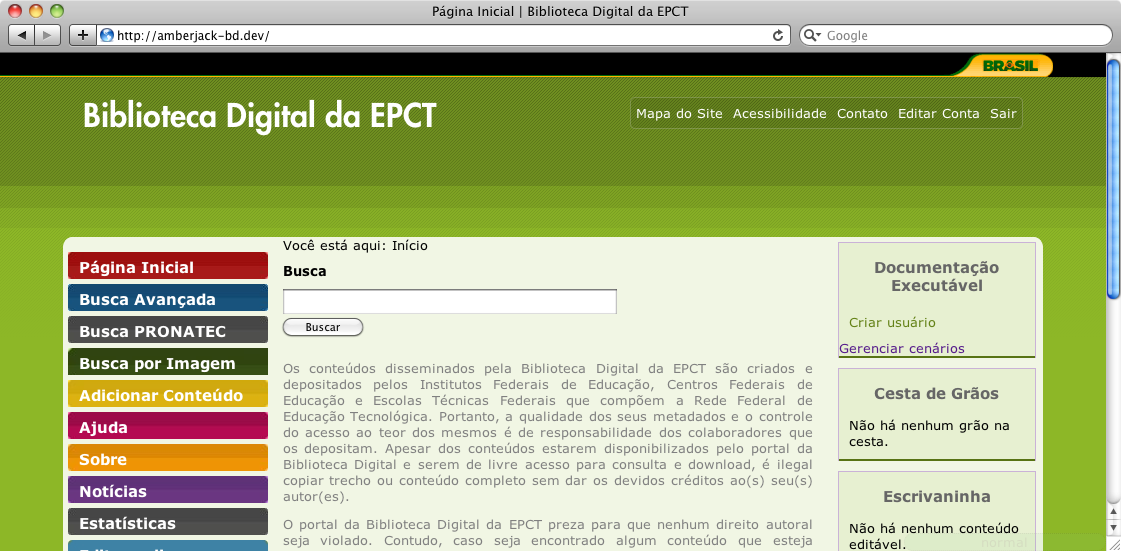
\includegraphics[width=0.9 \textwidth]{figuras/tour_1}
    \caption{Página incial do projeto Biblioteca Digital}
    \label{tour_1}
\end{figure}

No portlet referente a documentação executável, pode-se visualizar os vários cenários existentes e a opção de gerenciá-los.

\pagebreak
Clicando sobre a opção “Gerenciar cenários”, conforme apresentado na Figura \ref{tour_2}, pode-se criar, alterar ou excluir cenários.

\begin{figure}[ht]
    \centering
    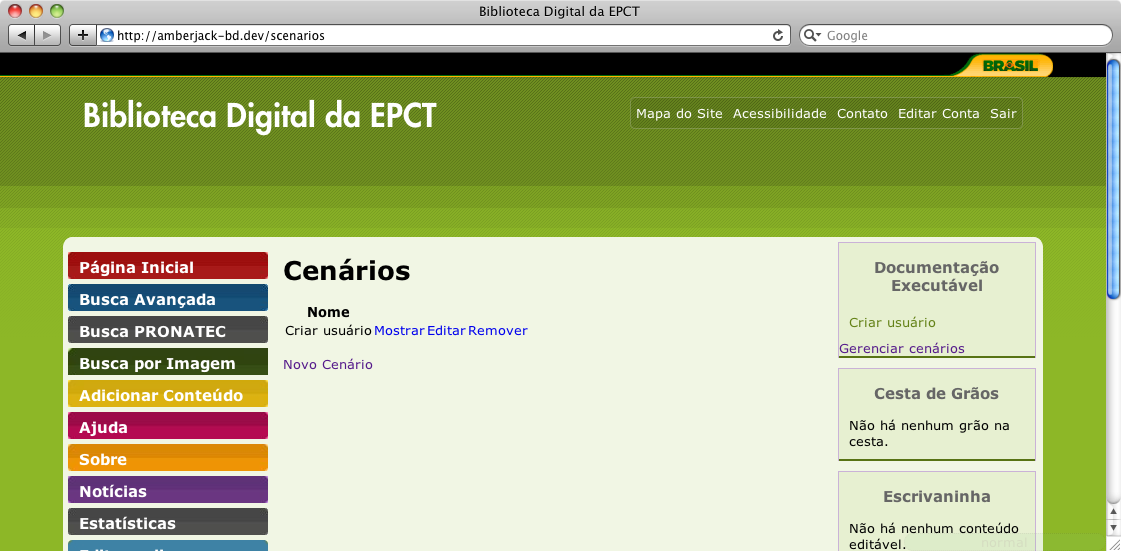
\includegraphics[width=0.9 \textwidth]{figuras/tour_2}
    \caption{Interface de gerenciamento de cenários}
    \label{tour_2}
\end{figure}

Na Figura \ref{tour_3}, pode-se observar a criação de um novo cenário que terá o objetivo de validar a funcionalidade de Busca Avançada da BD.

\begin{figure}[ht]
    \centering
    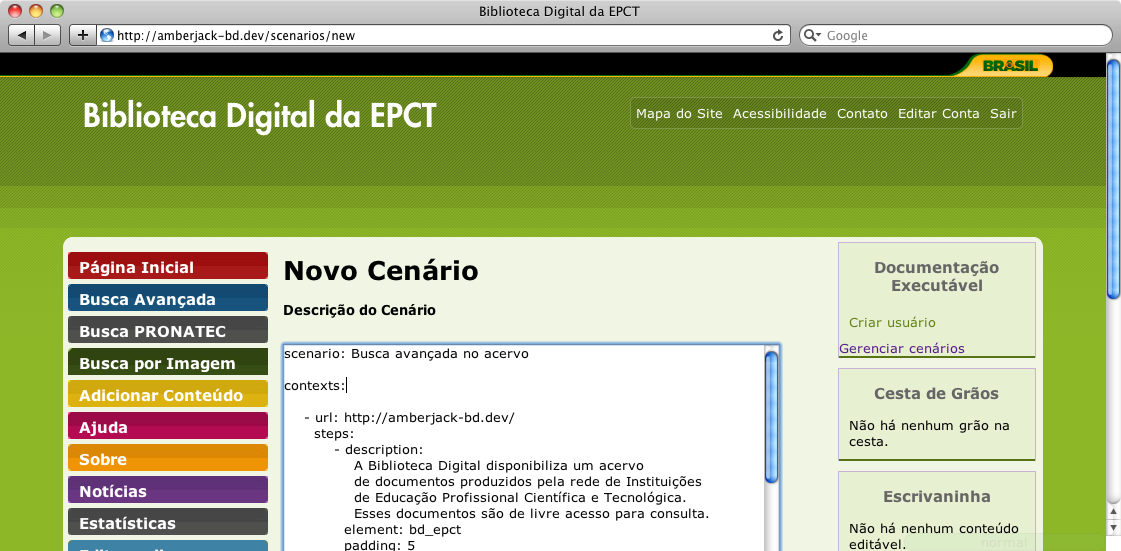
\includegraphics[width=0.9 \textwidth]{figuras/tour_3}
    \caption{Criação de um novo cenário}
    \label{tour_3}
\end{figure}

Ainda na Figura \ref{tour_3}, pode-se observar o campo “Descrição do Cenário”, onde foi inserido a descrição dos passos necessários para a execução do cenário, que precisa atender ao padrão YAML, conforme descrito no  tópico \ref{sec:yaml} do referencial teórico.

Cabe ressaltar que a atual interface não critica o atendimento do padrão, sendo essa crítica do formato, uma funcionalidade prevista para  trabalhos futuros.

Após a criação do cenário, o link para a execução do mesmo ficará disponível no portlet “Documentação Executável”. Ao clicar neste link, o usuário será redirecionado para a primeira página da funcionalidade avaliada pelo cenário que será então executado (Figura \ref{tour_4}).

\begin{figure}[ht]
    \centering
    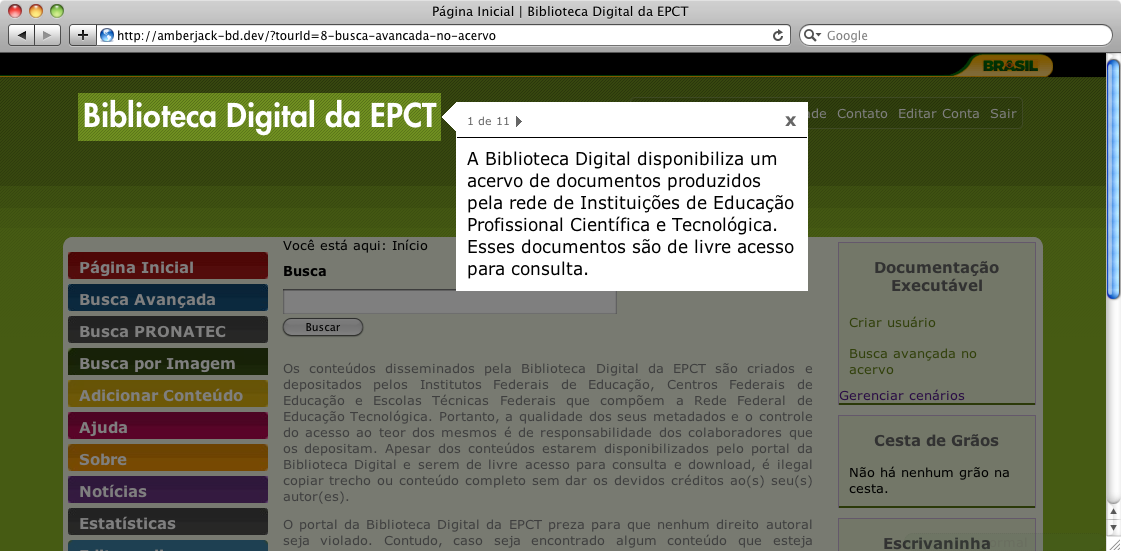
\includegraphics[width=0.9 \textwidth]{figuras/tour_4}
    \caption{Início da execução do cenário}
    \label{tour_4}
\end{figure}

A execução dos cenários, conforme descrito neste trabalho, visa trazer ao usuário o entendimento e a validação das funcionalidades existentes no sistema. Como pode ser observado na Figura \ref{tour_4}, serão apresentados balões numerados e iluminados na interface do sistema, enquanto o restante da interface permanece obscurecida em segundo plano. Pode-se observar também, no canto superior esquerdo do balão, a numeração do passo sendo executado e a totalidade de passos do cenário. O usuário ainda pode retroceder ou avançar o passo atual através dos links em formato de seta para a esquerda e direita, respectivamente, que se encontram ao lado da numeração do passo.

No canto superior direito, pode-se encontrar um link para a interrupção da execução do cenário, sinalizado por um “x”.

A execução do cenário, é portanto, composta por vários passos sequenciais que precisam ser executados para que a funcionalidade seja avaliada. Em cada um destes passos, a ferramenta guia o usuário através das páginas do sistema, executando as ações necessárias para a demonstração da funcionalidade. Durante o tempo em que o cenário estiver em execução, os elementos da interface do sistema ficarão indisponíveis para a interação do usuário, que deverá usar os links oferecidos no balão do NSI-BD-Tour.

Quando um passo, representado por um balão na interface, requer a execução de alguma ação interativa do usuário, um botão com o dizer “PRESSIONE PARA EXECUTAR” ficará disponível logo abaixo do texto descritivo do passo. Ao ser pressionado pelo usuário, esse botão simulará a ação descrita, executando automaticamente o passo, como por exemplo o clique de um link ou o preenchimento de um campo.

Na Figura \ref{tour_5}, pode-se obervar a execução do passo 4, em que o preenchimento de um campo de texto é requerido pela funcionalidade e executado pela ferramenta.

\begin{figure}[ht]
    \centering
    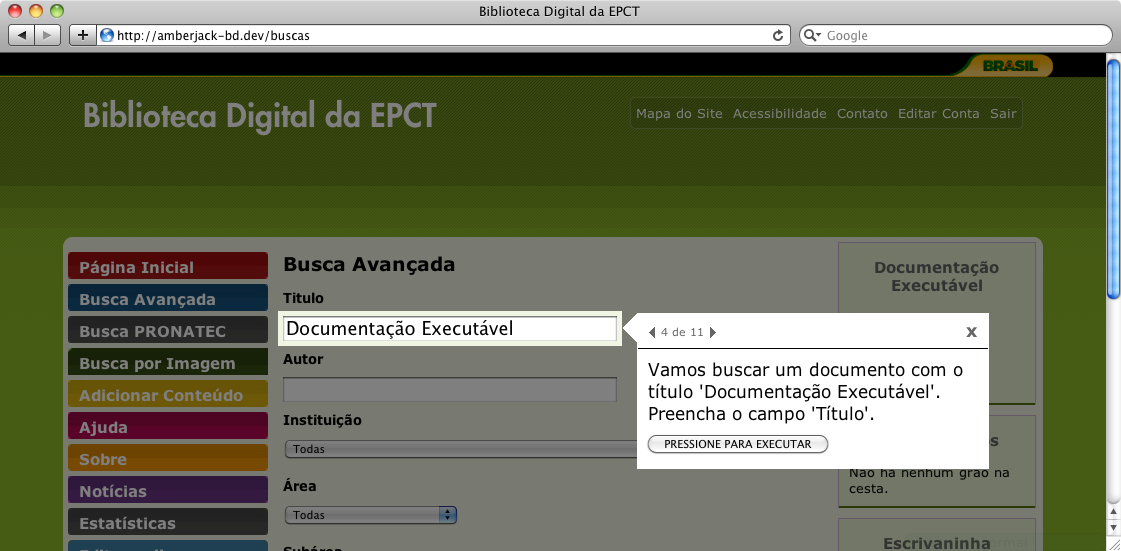
\includegraphics[width=0.9 \textwidth]{figuras/tour_5}
    \caption{Execução do passo 4 do cenário “Busca Avançada”}
    \label{tour_5}
\end{figure}

Após a execução da busca, é apresentado uma página com a listagem dos documentos recuperados pela mesma, como pode ser observado na Figura \ref{tour_6}. Neste caso, a Biblioteca Digital recuperou apenas um resultado, o documento “Documentação Executável”.

\begin{figure}[ht]
    \centering
    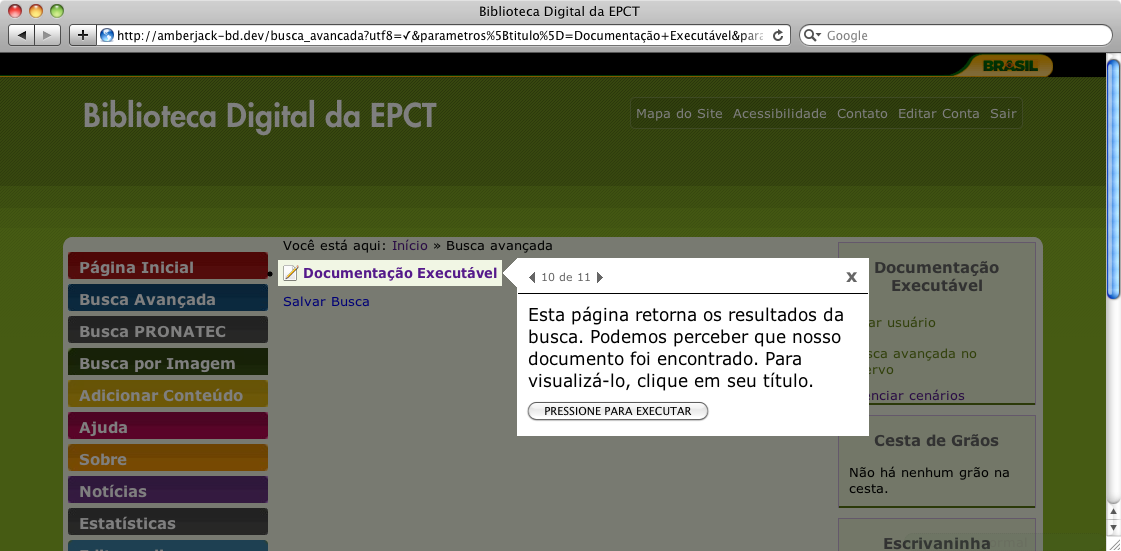
\includegraphics[width=0.9 \textwidth]{figuras/tour_6}
    \caption{Passo demonstrando a página de resultados da Busca Avançada}
    \label{tour_6}
\end{figure}

\pagebreak

Por fim, caso algum dos documentos retornados pela busca seja de interesse do usuário, ele pode abrir a página de visualização do documento (Figura \ref{tour_7}), onde além de informações mais detalhadas sobre o mesmo, outras funcionalidades são oferecidas, como por exemplo o download do documento ou possibilidade de favoritá-lo.

\begin{figure}[ht]
    \centering
    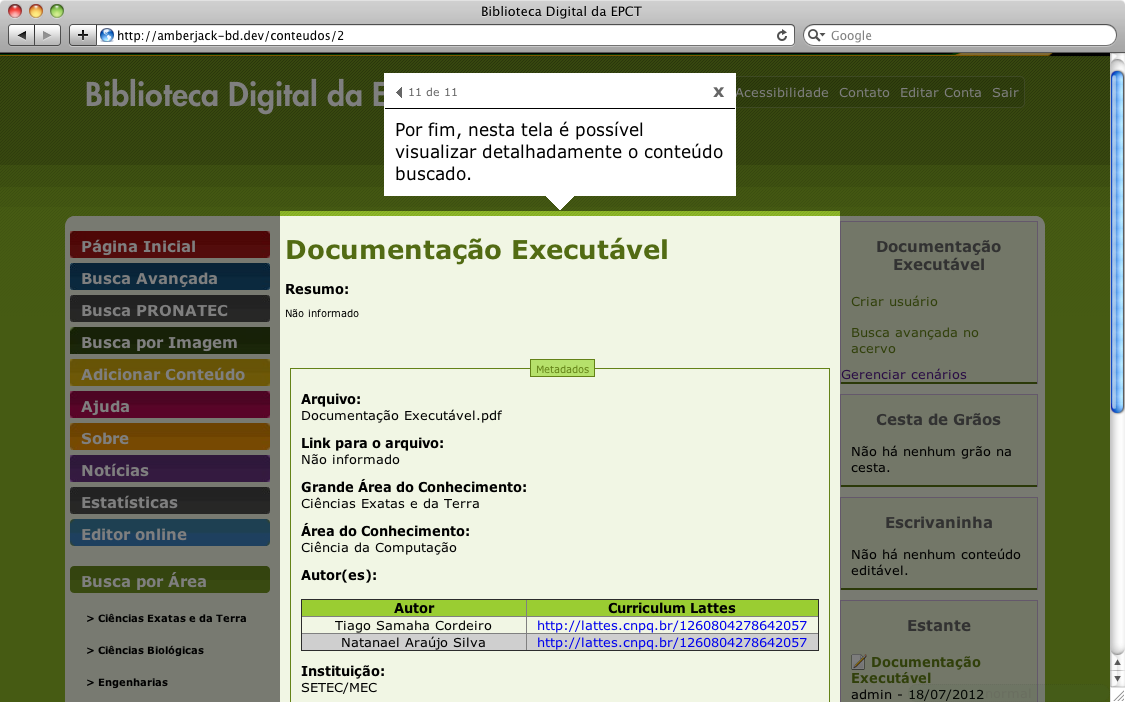
\includegraphics[width=0.9 \textwidth]{figuras/tour_7}
    \caption{Página de visualização do documento recuperado pela busca}
    \label{tour_7}
\end{figure}

Conforme descrito na apresentação do uso da ferramenta, o usuário é conduzido em um processo previamente especificado na descrição do cenário, possibilitando o seu treinamento conforme esperado.

As características da funcionalidade foram descritas, anunciadas ao usuário, possibilitando identificar detalhes de uma forma prática e interativa. Neste ponto, torna-se evidente a vantagem sobre a uma documentação tradicional, na qual as funcionalidades descritas podem não trazer ao leitor o real entendimento e experiência necessárias ao uso.

Como a execução dos cenários utiliza o sistema real, neste caso a Biblioteca Digital, pode-se garantir que esta forma de documentação guarda um sincronismo com a implementação real do sistema superior a outras formas de documentação tradicionais que normalmente perdem sincronismo deixando o sistema legado.

Adicionalmente, cada cenário descrito e executado pela ferramenta NSI-BD-Tour, está sendo validado no sentido real de teste de aceitação. Desta forma, quaisquer alterações que venham ser aplicadas no sistema, estarão sendo monitoradas e sinalizadas pela ferramenta. Este comportamento garante aos desenvolvedores e usuários, caso os cenários sejam executados com sucesso, que as funcionalidades cobertas por estes estejam em condições de uso.